\documentclass[border=2pt]{standalone}
\usepackage{tikz}
\usetikzlibrary{positioning,arrows.meta}
\begin{document}
\sffamily\footnotesize
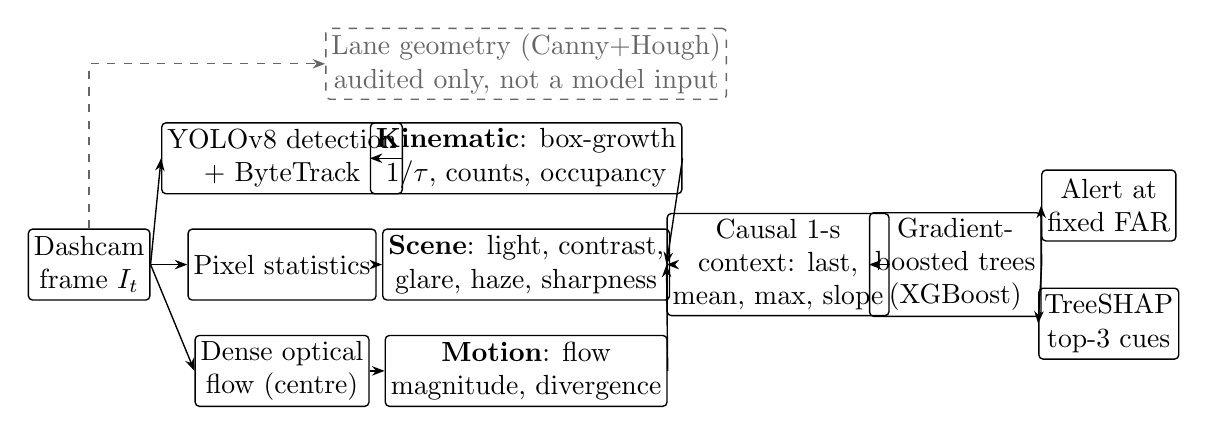
\begin{tikzpicture}[
  box/.style={draw, rounded corners=1.5pt, align=center, minimum height=9mm, inner sep=2pt, line width=0.5pt},
  arr/.style={-{Stealth[length=1.6mm]}, line width=0.5pt}]
% column x positions
\def\xa{0} \def\xb{2.45} \def\xc{5.55} \def\xd{8.75} \def\xe{11.0} \def\xf{12.95}
\node[box, minimum width=14mm] (cam) at (\xa,0) {Dashcam\\frame $I_t$};
\node[box, minimum width=21mm] (det) at (\xb,1.35) {YOLOv8 detection\\+ ByteTrack};
\node[box, minimum width=21mm] (pix) at (\xb,0) {Pixel statistics};
\node[box, minimum width=21mm] (flo) at (\xb,-1.35) {Dense optical\\flow (centre)};
\node[box, minimum width=27mm] (kin) at (\xc,1.35) {\textbf{Kinematic}: box-growth\\$1/\tau$, counts, occupancy};
\node[box, minimum width=27mm] (scn) at (\xc,0) {\textbf{Scene}: light, contrast,\\glare, haze, sharpness};
\node[box, minimum width=27mm] (mot) at (\xc,-1.35) {\textbf{Motion}: flow\\magnitude, divergence};
\node[box, minimum width=27mm, dashed, text=black!60, draw=black!60] (lane) at (\xc,2.55) {Lane geometry (Canny+Hough)\\audited only, not a model input};
\node[box, minimum width=17mm] (ctx) at (\xd,0) {Causal 1-s\\context: last,\\mean, max, slope};
\node[box, minimum width=15mm] (gbt) at (\xe,0) {Gradient-\\boosted trees\\(XGBoost)};
\node[box, minimum width=15mm] (alert) at (\xf,0.75) {Alert at\\fixed FAR};
\node[box, minimum width=15mm] (shap) at (\xf,-0.75) {TreeSHAP\\top-3 cues};
\foreach \n in {det,pix,flo} \draw[arr] (cam.east) -- (\n.west);
\draw[arr, black!60, dashed] (cam.north) |- (lane.west);
\draw[arr] (det) -- (kin); \draw[arr] (pix) -- (scn); \draw[arr] (flo) -- (mot);
\foreach \n in {kin,scn,mot} \draw[arr] (\n.east) -- (ctx.west);
\draw[arr] (ctx) -- (gbt);
\draw[arr] (gbt.east) -- (alert.west); \draw[arr] (gbt.east) -- (shap.west);
\end{tikzpicture}
\end{document}
